\section{设计主题}
本毕业设计的研究主题是：“\Title”，
旨在探索如何从已有的带材质模型和对应的白模出发，
实现自动化材质生成与迁移。
传统的材质生成方法多依赖于从单张图片或多视图生成模型表面效果，
而本研究更侧重于模型层面的材质推断：即利用已有带材质的模型作为参考，
结合白模的几何信息，生成符合其形态和结构的材质贴图，
实现白模到完整材质模型的自动转换。

此外，本研究不仅关注算法层面的实现与优化，
还将搭建一个基于 Web 的交互平台，
为用户提供模型上传、材质生成与结果预览等功能，
从而使相关技术能够以直观、便捷的形式被用户使用，
提升系统的实用性与交互体验。

\subsection{相关研究}
近年来，随着深度学习与生成式人工智能的发展，
三维模型纹理生成技术取得了显著进展。
传统三维建模流程中，纹理通常需要设计人员手动绘制或在专业软件中进行贴图，
这一过程不仅耗时较长，而且对设计经验要求较高。
因此，研究者开始探索利用深度学习方法自动生成三维模型纹理，
以提高三维资产生产效率。

在早期研究中，一些方法尝试将二维图像生成技术应用到三维模型纹理生成任务中。
例如 Kato 等人提出可微分渲染框架，
使得二维图像空间中的损失函数能够反向传播到三维网格纹理，
从而实现基于深度学习的三维纹理优化 \cite{kato2018neural}。
随后，一些研究进一步将卷积神经网络应用于三维纹理生成任务，
通过在 UV 纹理空间中学习纹理分布，
实现从几何结构到纹理贴图的自动生成 \cite{pavllo2020convolutional}。
这些方法将三维纹理生成问题转化为二维图像生成或优化问题，
为后续基于深度生成模型的三维纹理生成研究奠定了基础。

随着生成模型的发展，
扩散模型逐渐成为三维纹理生成的重要技术路径。\cite{ho2020denoising}
例如 TexFusion 方法，
通过文本引导的扩散模型对多视角渲染图像进行去噪，
并将生成结果融合到统一的 UV 纹理空间中，
从而生成具有较高一致性的三维纹理贴图 \cite{Cao_2023_ICCV}。
该方法基于 Score Distillation Sampling（SDS）从预训练扩散模型中提取梯度信号，
对三维纹理进行迭代优化，
并通过多视角一致性约束有效缓解纹理错位问题。

随后，一些研究进一步将扩散模型与可微渲染技术结合。
例如 TEXTure\cite{richardson2023texture}、 Text2Tex\cite{chen2023text2tex}等方法通过在多视角渲染图像上迭代生成纹理，
并将生成结果逐步回投到模型表面，
实现了更加稳定且细节丰富的三维纹理生成。
这类方法通过结合几何信息与图像生成能力，
显著提升了纹理的真实感与空间一致性。

在最新研究中，一些工业级系统开始将大规模生成模型引入三维纹理生成流程。
Hunyuan3D 2.0 通过多模态输入与扩散生成框架相结合，
利用多视角图像生成与三维重建技术生成具有一致纹理的三维模型。\cite{zhao2025hunyuan3d}
除此之外，
也有研究探索直接三维生成的方法，
他们使用结构化三维潜空间表示，
使模型能够直接生成三维形状与纹理，
从而避免多视角优化过程，
提高生成效率与可扩展性。\cite{xiang2025structured}

综上所述，当前三维纹理生成技术遵循
“二维纹理映射—多视角一致性优化—扩散模型驱动生成”
这一演进路径不断深化。
通过深度整合生成式扩散概率模型、
可微渲染以及多视角注意力融合技术，
研究者已逐步实现从多模态输入（文本或图像）
向三维几何表面纹理的高质量自动化映射。
这些技术范式的变革，不仅大幅提升了三维内容生产的自动化水平，
也为本研究中基于参考模型的风格解耦与材质迁移方法
奠定了坚实的技术基础与理论框架。

\subsection{设计案例}
在三维资产生成与材质迁移领域，学术算法的突破为功能实现提供了核心驱动，
而商业化平台的演进则在用户体验、交互链路以及实时反馈机制方面积累了大量成熟的设计范式。

本节旨在脱离底层算法实现，
重点剖析国内外三个代表性平台的界面逻辑与交互策略，
为本系统的功能布局与交互流程提供设计依据.

\subsubsection{腾讯混元3D}
腾讯混元3D是腾讯推出的三维内容生成平台，支持用户通过文本描述或图像输入快速生成三维模型及其材质。
该平台依托腾讯混元大模型体系，实现了从多模态输入到三维资产生成的自动化流程，
能够在较短时间内完成模型结构重建与纹理生成。
与传统三维建模软件需要复杂建模操作不同，
混元3D更强调“生成式内容生产”的理念，
通过 AI 自动推理完成大部分建模与材质生成任务。

在界面设计方面，混元3D更加注重任务流程的清晰性，
整体界面围绕生成流程进行组织，
用户只需完成输入内容、触发生成以及查看结果三个主要步骤。
平台在页面左侧或输入区域提供文本或图像输入框，
用户上传参考图片或输入描述后，
系统即可自动调用后台模型完成三维生成任务。

在结果展示阶段，系统会在页面中提供三维模型的实时预览窗口，
用户可以对生成模型进行基本的旋转、缩放与视角观察，
以检查模型整体结构与材质效果。
同时，平台还会显示模型生成状态、生成时间以及部分基础信息，
使用户能够直观了解生成结果。

在交互设计上，混元3D更加侧重于“生成流程驱动”的使用体验，
用户无需进行复杂的模型编辑操作，
而是通过简单的输入与生成步骤获得三维资产。
生成完成后，平台支持将模型导出为常见的三维格式，
便于在游戏开发、虚拟场景搭建或数字内容创作中进一步使用。
这种以自动化生成流程为核心的设计模式，
体现了 AI 三维生成平台在降低创作门槛方面的重要发展方向。
\begin{figure}[htbp]
    \centering
    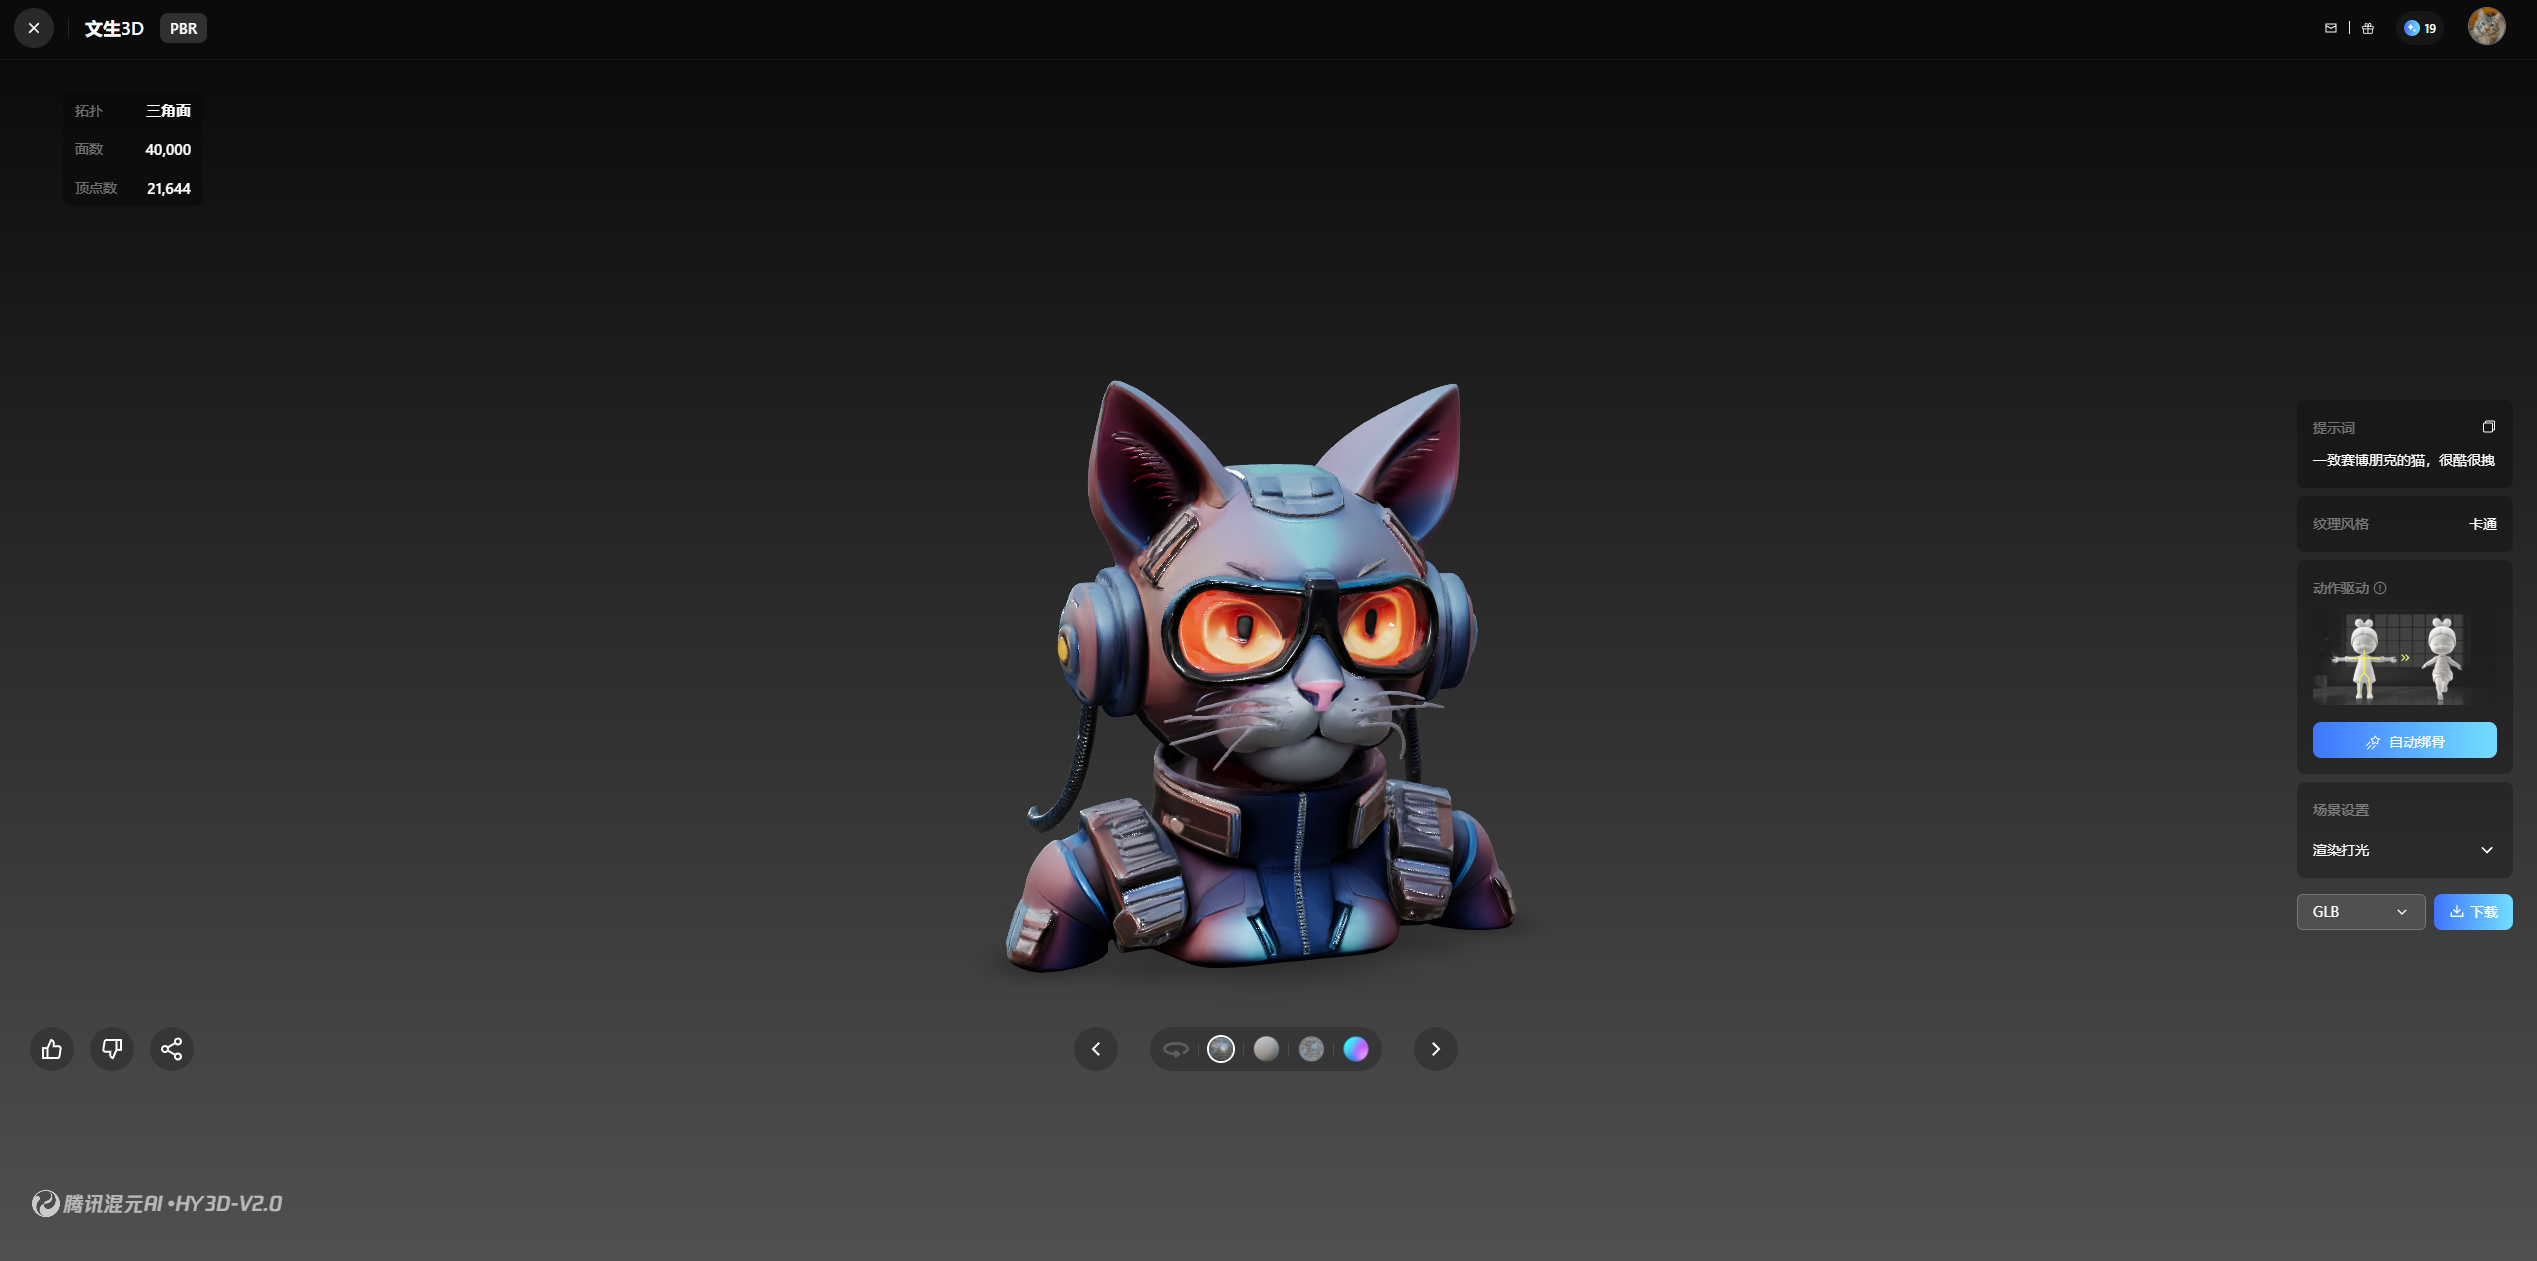
\includegraphics[width=0.8\textwidth]{figure/comparison/topic/hunyuan3d.png}
    \caption{腾讯混元3D 平台界面}
    \label{fig:hunyuan3d}
\end{figure}

\subsubsection{Tripo}
Tripo 是近年来发展较快的 AI 三维内容生成平台之一，
其核心功能涵盖从文本描述或二维图像输入到三维模型及其材质的自动化生成。
与传统三维建模软件（如 Blender 或 3ds Max）相比，
Tripo 更强调基于 Web 的轻量化交互体验，
用户无需安装复杂的本地软件，
即可在浏览器环境中完成模型生成、实时预览以及基础管理操作，
显著降低了三维内容创作的技术门槛。

在界面设计方面，Tripo 采用以三维视窗为核心的可视化布局结构，
生成结果会直接展示在中心的三维视图中，
用户可以通过鼠标交互对模型进行旋转、缩放和视角调整，
以多角度观察生成效果。
同时，平台在侧边栏区域提供参数设置与生成控制功能，
用户能够查看生成过程相关信息并对部分参数进行调整。

此外，平台还提供了模型导出与分享功能，
支持将生成的三维资产以常见格式导出，
从而便于在 Unity、Unreal Engine 等三维开发环境中继续使用。
这种以可视化结果为核心的交互设计模式，
使用户能够在较短时间内完成从二维信息到三维模型的生成与查看过程，
体现了当前 AI 三维生成平台在交互体验与生产效率方面的发展趋势。
\begin{figure}[htbp]
    \centering
    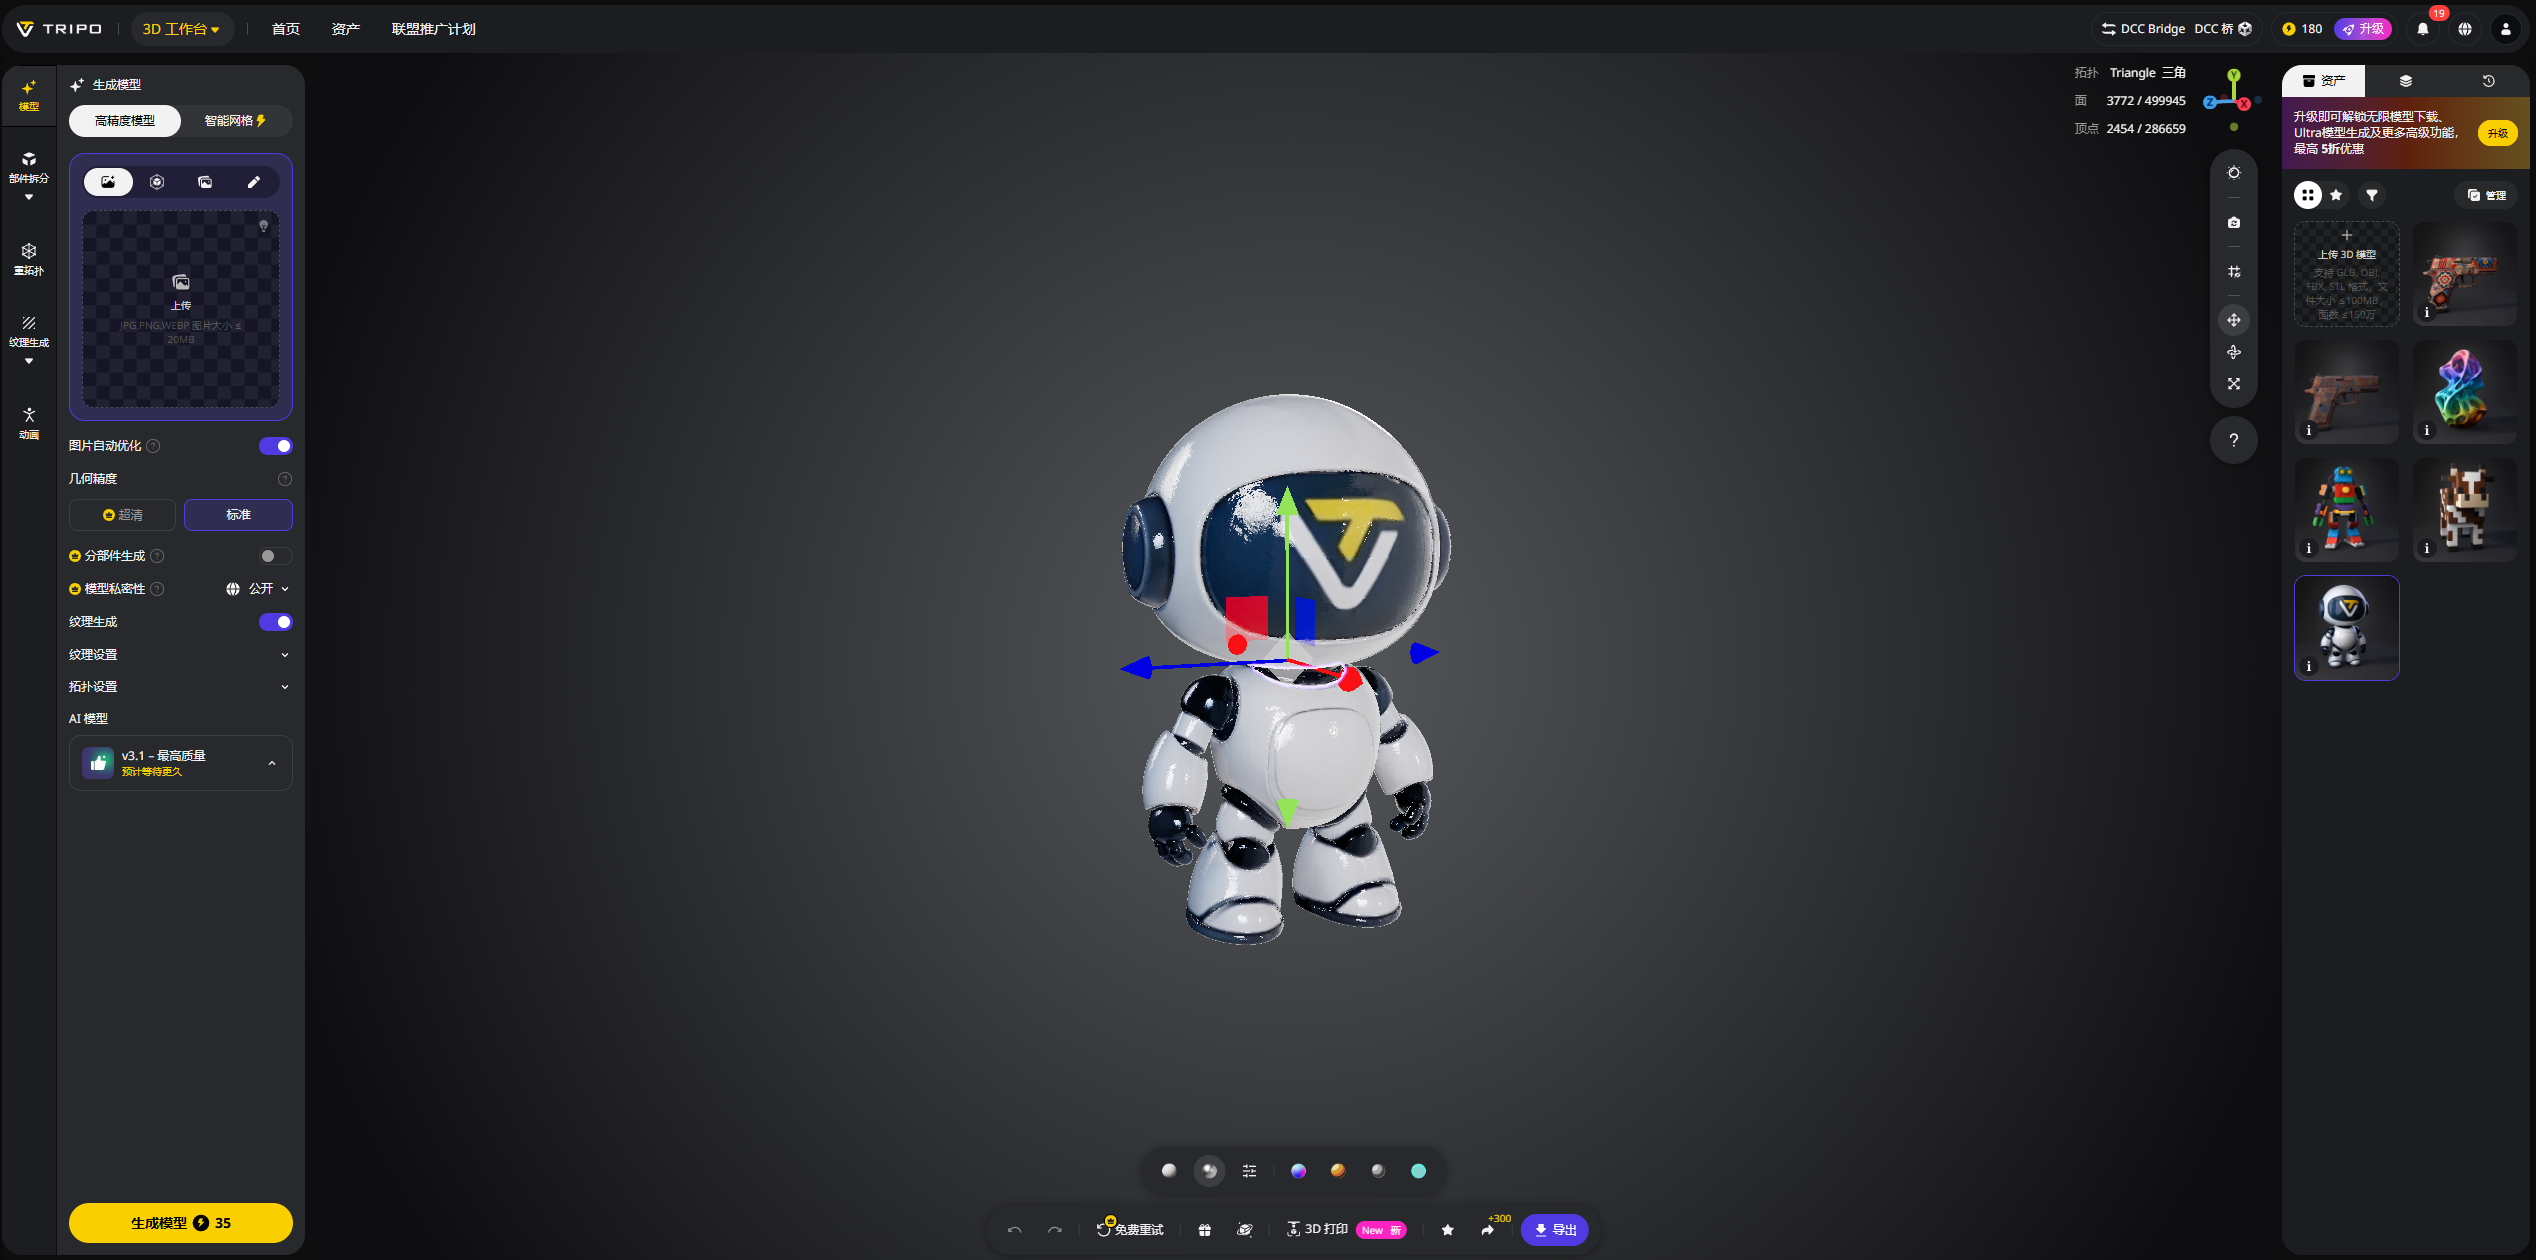
\includegraphics[width=0.8\textwidth]{figure/comparison/topic/tripo.png}
    \caption{Tripo 平台界面}
    \label{fig:tripo}
\end{figure}

\subsubsection{Meta SAM 3D}
Meta SAM 3D 是由 Meta AI Research 提出的单图三维重建系统，
其目标是通过视觉基础模型实现从单张二维图像到完整三维结构的自动重建。
该系统基于 Segment Anything 系列模型扩展而来，
能够从单张 RGB 图像中预测物体的几何形状、纹理信息以及空间布局，
从而生成完整的三维网格模型。与传统摄影测量方法需要多视角图像不同，
SAM 3D 仅依赖单张图像即可完成三维重建，
在复杂场景或遮挡情况下仍能够推断合理的三维结构。

在界面设计方面，SAM 3D 的在线演示平台整体结构较为简洁，
更接近研究型系统的实验界面。
页面主要由图像上传区域、生成控制区域以及三维预览窗口构成。
用户可以通过拖拽方式上传图片，
系统支持常见的 JPG、PNG 等图像格式，
随后通过点击生成按钮触发后台推理过程。 

在生成完成后，平台会在页面中展示交互式三维预览窗口，
用户可以对生成的模型进行基础的旋转、缩放和视角观察，
以查看模型的几何结构与纹理效果。
与商业化三维平台相比，
SAM 3D 的交互功能相对简化。

总体而言，SAM 3D 更偏向于研究驱动型的三维生成系统，
其界面设计以算法演示与实验验证为核心，
而非完整的生产工具链。
这种以“单图输入—自动推理—三维结果展示”为主的交互模式，
为后续商业化三维生成平台的发展提供了重要的技术基础。
\begin{figure}[htbp]
    \centering
    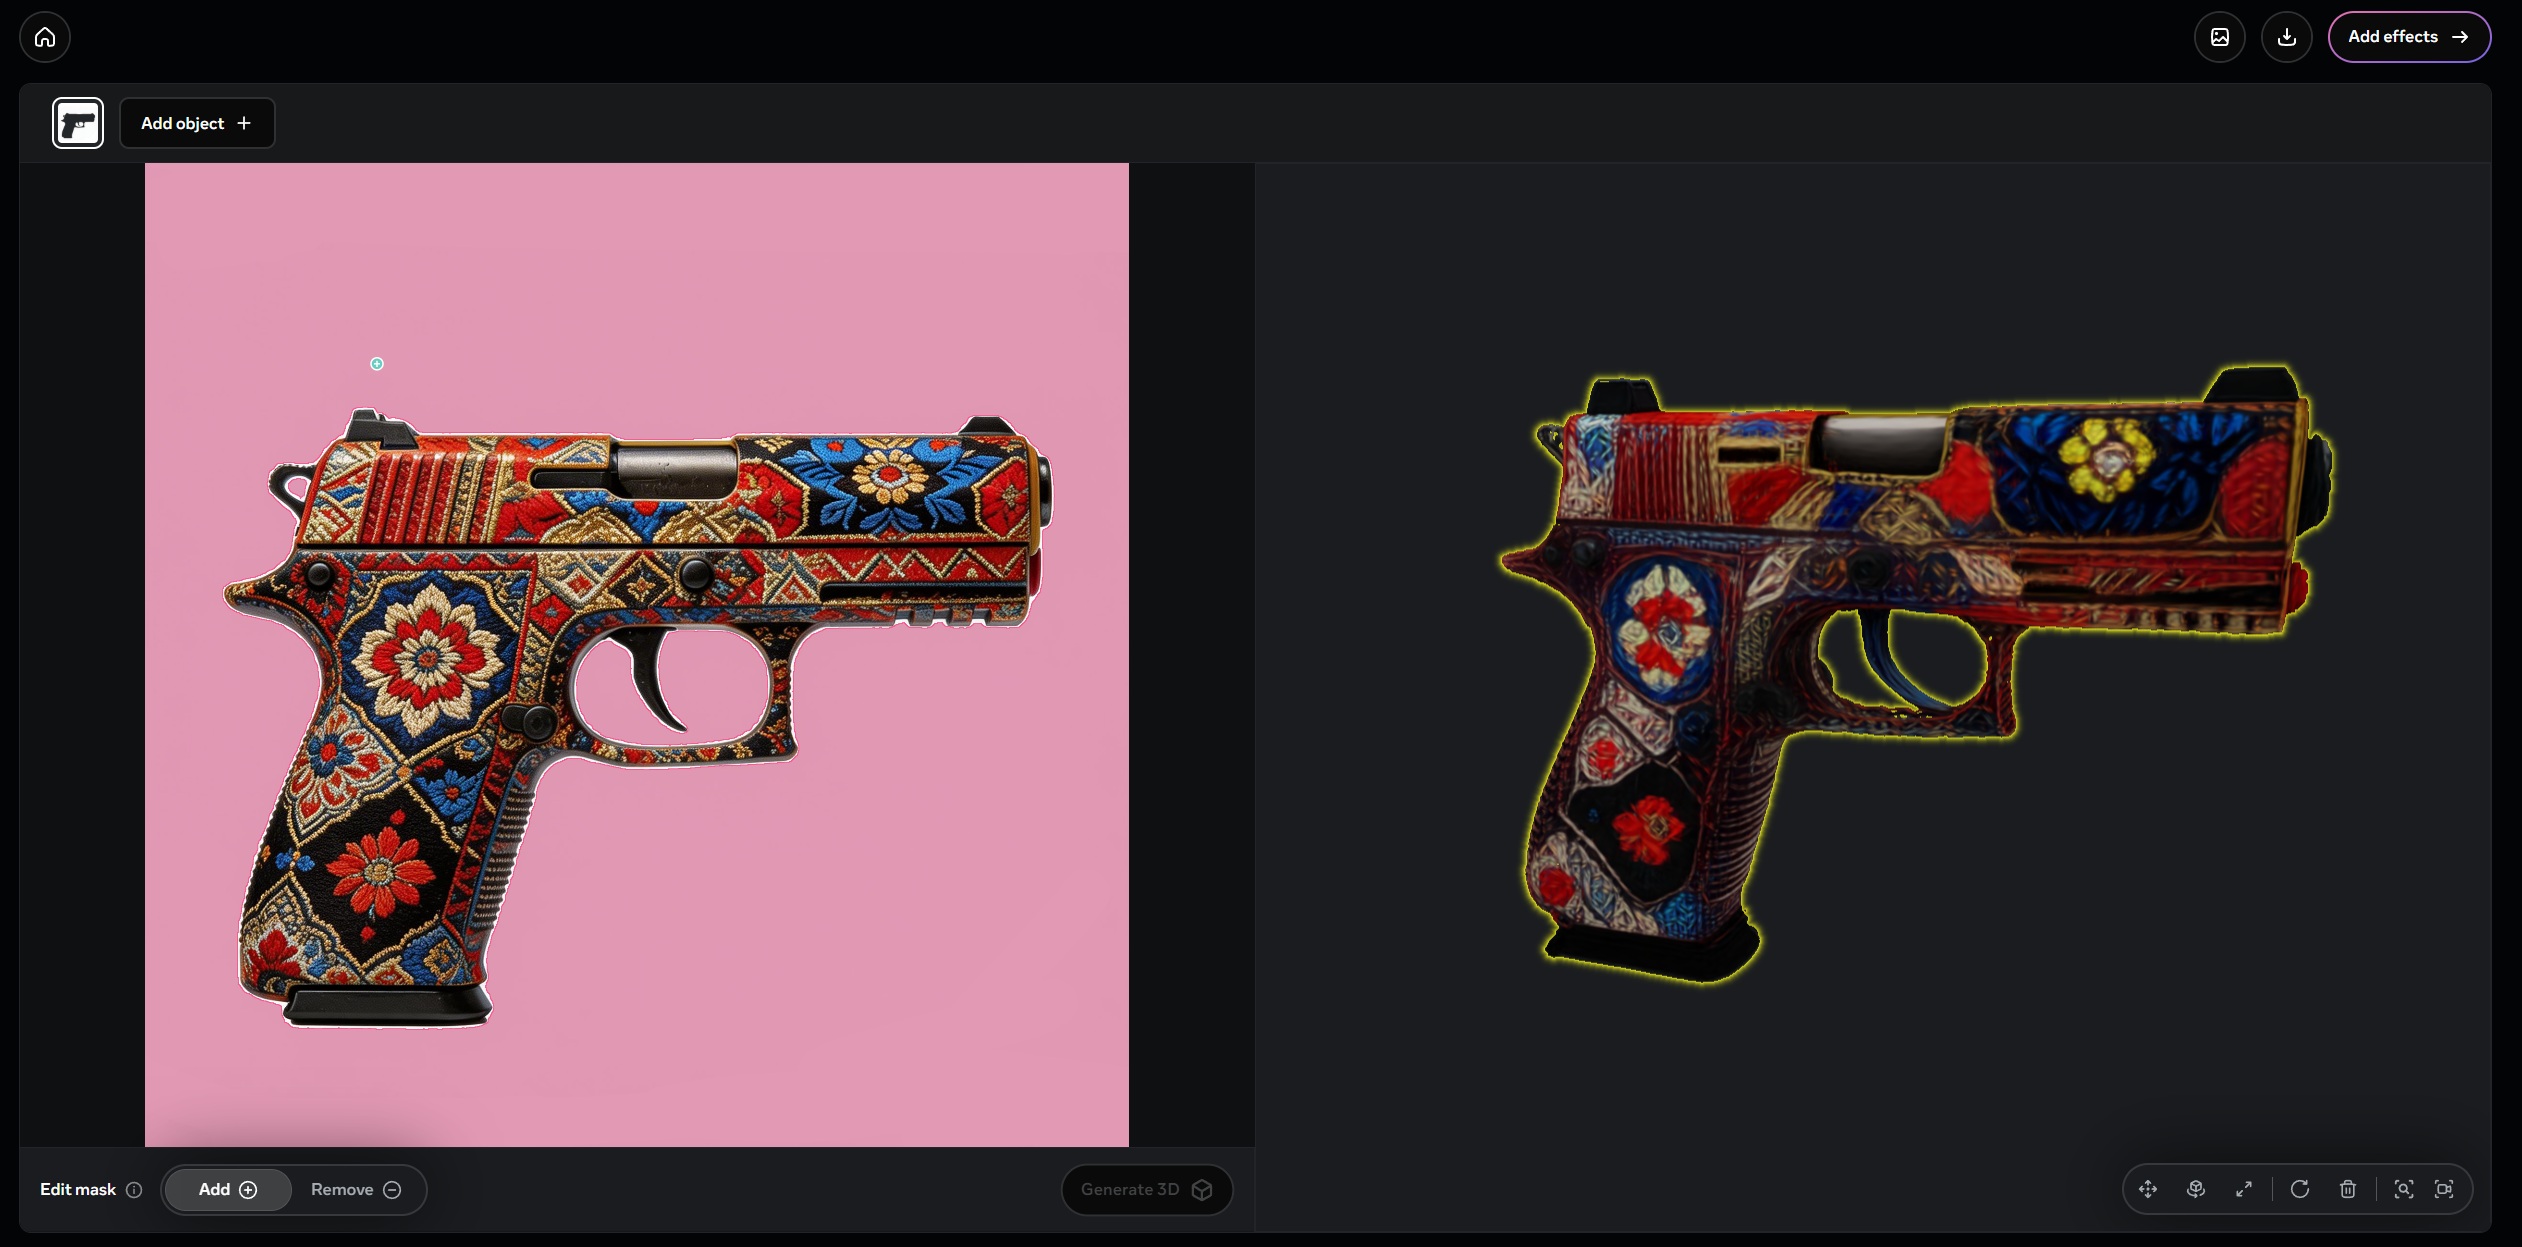
\includegraphics[width=0.8\textwidth]{figure/comparison/topic/sam3d.png}
    \caption{Meta SAM 3D 平台界面}
    \label{fig:sam3d}
\end{figure}

